\pagebreak
\section{Approach}

A system for the benchmarking of Networked Control Systems needs to be able to 
\todo[inline]{Explain what it needs}
Existing platforms take one of two approaches.
The first is a fully simulated approach, in which the plant, network and controller reside in a completely simulated environment.
This allows for unparalleled flexibility, as parts of the system can be swapped out or modified without greater difficulty.
However, this comes at the cost of realism, as these models are always approximations of reality; and time, as these simulations are often very computationally expensive.

The alternative is an approach using a testbed comprised of a \emph{physical} plant that interacts with a \emph{real} network and controller.
This of course allows for great realism, but provides very little flexibility in terms of the components of the system, limiting the approach to whatever plant, network and controller are available.

CLEAVE tries to mitigate the shortcomings of these approaches by walking the line between them.
We employ a third strategy based on having a real-time emulated representation of a control system interacting with a real network.
This allows for great flexibility when it comes to the components of the control system, as these are as easily switched out as in the fully simulated approach, while maintaining the realism of arguably the most complex and limiting component of an NCS, namely the network itself.

\begin{figure*}
    \centering
    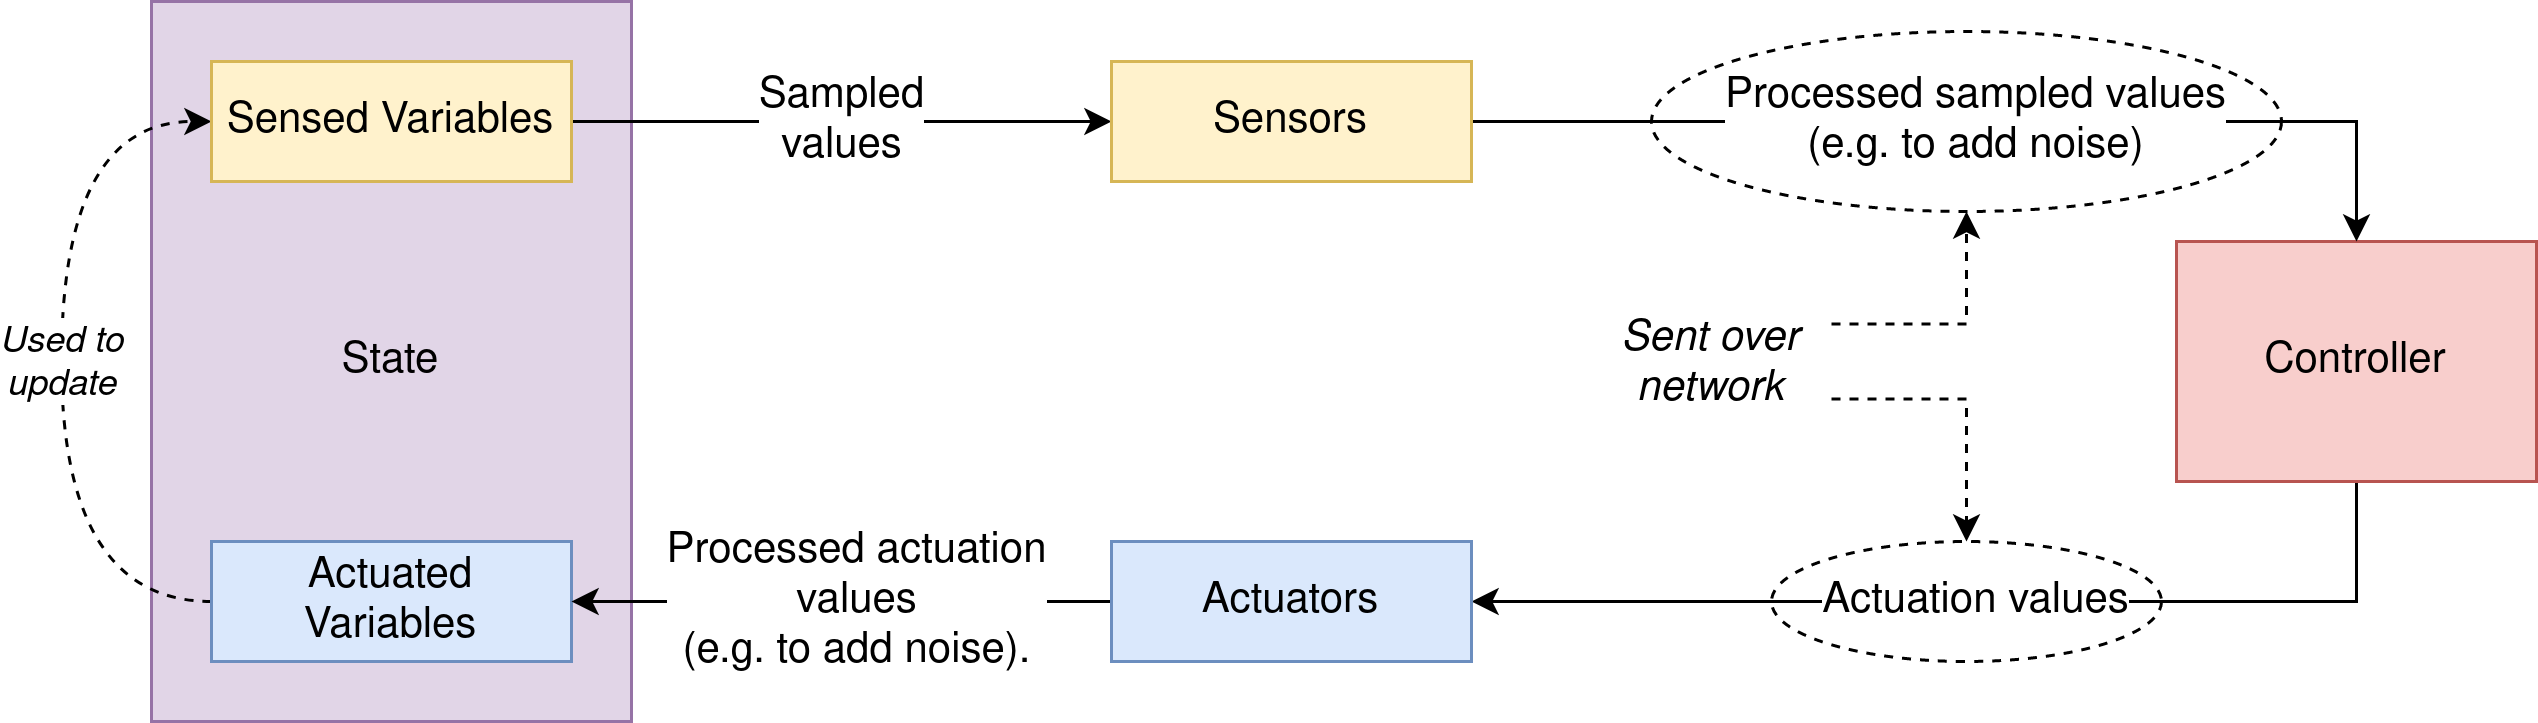
\includegraphics[width=\textwidth]{images/CLEAVE_NCS_structure.png}
    \caption{
        Structure of an emulated NCS on top of CLEAVE.
        The State object implements the discrete-time evolution of the Plant.
        For this purpose, it holds two sets of special variables; Actuated Variables and Sensed Variables.
        Actuated Variables are updated from the values obtained from the Actuator objects at the beginning of each time step.
        These are used to perform a time step update in the State, and update the values of the Sensed Variables.
        The values of the Sensed Variables are then, at the end of each time step, sampled and passed on to the Sensor objects, which in turn process them (for instance, to add noise) and send the processed values to the Controller.
        The Controller uses these values to calculate the new actuation commands and sends these to the Actuators.
        Finally, the Actuators process the actuation commands and hold the new values for the Actuated Variables until they are read at the next time step.
    }
\end{figure*}

Concretely, in the following we describe the procedure for benchmarking an NCS on the CLEAVE framework:

\begin{enumerate}
    \item A discrete-time emulation of the target Plant is implemented.
    CLEAVE provides a simple API for this task in the form of an \emph{abstract base class} \mintinline{Python}{class State(abc.ABC)} users need to extend.
    This class provides an abstract method \mintinline{Python}{State.advance(delta_t: float)} which is called by CLEAVE on each emulation time step with the number of seconds since the previous iteration.
    Additionally, the class provides functionality for the assigning special instance variables that can be sampled from or actuated upon during the emulation.

    \item A Controller for the Plant is developed.
    Once again, CLEAVE provides an API for this in the form of the \mintinline{Python}{class Controller(abc.ABC)} abstract base class.
    Users need to extend this class and implement the \mintinline[breaklines]{Python}{Controller.process(sensor_values: Mapping) -> Mapping} method, which will be called with a mapping from property names to sampled values and should return a mapping from property names to actuated values.
    
    \item A configuration file for the benchmarking run is written.
    Deployments in CLEAVE are configured through fully-featured Python scripts which simply need to define a number of required (and some optional) top-level variables.
    These top-level variables include, for instance, a \mintinline[breaklines]{Python}{state} variable pointing to an instance of the target Plant emulation implementation and the name of the Controller class to use for the run, among other emulation parameters.
    
\end{enumerate}

\section{The CLEAVE Framework}\label{sec:cleave}

CLEAVE (\emph{ControL bEnchmArking serVice on the Edge}) is our framework for quick, robust, and repeatable benchmarking of networked control systems.
CLEAVE tackles this challenge through a number of key design decisions that we will discuss in the following.

\begin{description}[wide]
    \item[Emulation approach.] 
    Existing benchmarking platforms for NCS either take a fully simulated approach --- running plant, network, and controller inside a completely simulated environment --- or one requiring an actual physical plant that interacts with a real network and controller.
    CLEAVE walks the line between these two approaches, employing a strategy based on having a real-time emulated representation of a Plant interact with the real network and controller.
    \item[Plant- and Controller-agnosticism.] 
    CLEAVE makes as few assumptions as possible about the inner workings of both the Plant and the Controller. 
    The only requirements for a system to be able to be emulated in CLEAVE are
    \begin{enumerate*}[itemjoin*={{ and }}]
        \item that its behavior can be described in a discrete-time fashion;
        \item that its state and the actions performed on it can be described by a finite number of scalar and/or vector variables.
    \end{enumerate*} 


    \item[API based on well-defined components.]
    The previously mentioned agnosticism is achieved through careful abstraction of the the system into an API based around the following components:
    \begin{itemize}
        \item A \texttt{State} object, which implements the discrete-time evolution of the physical system being controlled.
        This object also holds a number of named properties that can be measured or actuated upon.
        \item An arbitrary number of \texttt{Sensor} objects which measure named properties of the \texttt{State}, and potentially transform them (for instance, to add noise).
        \item A \texttt{Controller} object which receives values of named properties processed by the \texttt{Sensor} objects and returns new values for the named properties of the \texttt{State} that can be actuated upon.
        \item Finally, an arbitrary number of \texttt{Actuator} objects which receive the values generated by the \texttt{Controller} and process them before passing them on the \texttt{State}.
    \end{itemize}
    Users implement their desired behavior by extending the abstract base classes defining these components provided by the framework.

    \item[Plain Python configuration.]
    As mentioned above, users implement their desired behavior for the core components by extending classes provided by the framework.
    This is done in configuration files written in full-featured Python simply defining a number of required top-level variables and which are then passed to the main script provided with CLEAVE.
    This allows for easy configuration of arbitrarily complex emulations.
    
\end{description}

\begin{figure}
    \centering
    \includegraphics[width=3cm]{example-image-a}
    \caption{Execution flow of a time step in CLEAVE.}
\end{figure}
    
\begin{listing}
    \begin{minted}[linenos=true,
        breaklines, 
        breakafter=d,
        fontsize=\small]{Python}
from cleave.api.plant import SimpleConstantActuator, SimpleSensor
from cleave.impl.inverted_pendulum import InvPendulumState

host = '0.0.0.0'  # address of dispatch server
port = 8080       # providing Controllers

# Controller parameters
controller_class = 'InvPendulumController'
controller_params = {'ref': 0.0}

# Plant emulation parameters 
tick_rate = 100
emu_duration = '30m'
state = InvPendulumState(fail_angle_rad=0.34)
output_dir = './plant_metrics'

sensors = [
    SimpleSensor('position', 100),
    SimpleSensor('speed', 100),
    SimpleSensor('angle', 100),
    SimpleSensor('ang_vel', 100),
]

actuators = [
    SimpleConstantActuator(initial_value=0, prop_name='force')
]
    \end{minted}
    \caption{
        Example configuration file.
        Users are simply required to define a number of top-level variables, but are otherwise free to include arbitrary code.
        This allows for the easy extension of emulations.
    }
    \label{lst:config}
\end{listing}
